% DO NOT COMPILE THIS FILE DIRECTLY!
% This is included by the other .tex files.

\begin{frame}[t,plain]
\titlepage
\end{frame}

\begin{frame}
    \frametitle{Objectives of this module}
    \begin{itemize}
        \item How evidences can be useful for defense
        \item Why is contextualisation important
        \item What options do we have in MISP
        \item Best practises to encode and contextualise
        \item How can context be leveraged
        \item How to structure non-technical information
        \begin{itemize}
            \item Practical case: Conti analysis
        \end{itemize}
    \end{itemize}
\end{frame}

\section{How evidences can be useful for defense}
\begin{frame}
    \frametitle{How evidences can be useful for defense}
    The most common recommendations to protect people and assets from cyber attacks are usually:
    \begin{enumerate}
        \item Maintaining softwares up to date
        \item Staff awareness
        \item Reliable Backups
        \item Endpoints protection tools (IDS or SIEM)
    \end{enumerate}

    \note[item]{An Intrusion Detection System (IDS) is a tool that aims at detecting vulnerability exploits or suspicious activity against a server or a service.}
    \note[item]{A Security Information and Event Management (SIEM) allows centralise security alerts and events generated by endpoints and network devices.}

\end{frame}

\begin{frame}
    \frametitle{How evidences can be useful for defense}
    \begin{itemize}
        \item We can only help endpoints protection tools
        \item With the proper knowledge and methods, it is possible the maximize their accuracy and performance
    \end{itemize}

    These systems can rely on information extracted from
    \begin{itemize}
        \item Log files
        \item Network captures
        \item Disk forensic
        \item ...
    \end{itemize}
    
    However, from a MISP user perspective the hardest part in not to encode the raw evidences, it is to encode them so that they become \textbf{actionable}
\end{frame}

\section{Why is contextualisation important}
\begin{frame}
    \frametitle{Why is contextualisation important}
    \begin{itemize}
        \item Allow the distinction between information of interest and raw data
        \item provide guidance on how to use this information can be used for for protection
        \item Filter out noise from information unrelated from the use-case or activity
        \item Enable risk assessment based on attack type, TTP and threat actor
        \item Allow triage in large volume of data
        \item Allow false-positive management
    \end{itemize}

    \note[item]{Tactics, Techniques and Procedures (TTP) describe the context and a detailed description of the behavior taken by an actor}
\end{frame}

\begin{frame}
    \frametitle{Expectations of the recipients}
    Most common expectations of recipients when receiving information

    \begin{itemize}
        \item Being able to \textbf{consume} the data
        \item Find information is \textbf{relevant} for them and their partners
        \item Being able to \textbf{understand} the data and its classification
        \item Assess the \textbf{credibility}, likelyhood and origin of the data
    \end{itemize}

\end{frame}

\begin{frame}
    \frametitle{What do recipient hope to do with the data}
    Most common expectations of recipients for handling the data\\

    \begin{itemize}
        \item Being able to \textbf{filter} data efficiently for different use-cases
        \item Obtain as much \textbf{knowledge} out of the data as possible
        \item Know how this data was produced and where its \textbf{origin}
        \item Deduce why is the data \textbf{relevant} for them and how \textbf{critical} it is
    \end{itemize}
\end{frame}

\begin{frame}[fragile]
    \frametitle{Is context really that important?}
    
    \begin{itemize}
        \item Raw data \textbf{is} useful but useless if you don't know what it is about
        \item That's why it should carry how and why it's relevant
    \end{itemize}
    
    \begin{lstlisting}
1.2.3.9
137.221.106.104
28c643a1f69f9fca9481a4bc9f3f38f3
904afe59f6438848be96fd26fdeab01267070d25
evil.org
accounting.xlsx.exe
cat.jpg.exe
    \end{lstlisting}

    \begin{itemize}
        \item In MISP, all data intrinsically have some context
        \begin{itemize}
            \item \textbf{Type}: \texttt{ip-src} / \texttt{sha1} / \texttt{domain}
            \item \textbf{Category}: \texttt{network-activity} / \texttt{payload-delivery} / \texttt{external-analysis}
            \item \textbf{to\_ids}: \texttt{yes} / \texttt{no}
        \end{itemize}
    \end{itemize}

    
    \note[item]{The `to\_ids` flag is used to differentiate between indicators and supporting data. If the flag is set, it means the attribute is an indicator and is meant for protective tools.}
\end{frame}

\begin{frame}
    \frametitle{Is context really that important?}
    \begin{itemize}
        \item Sometime, more contextual information is not needed as data inherently convey its context:
        \begin{itemize}
            \item Tor exit nodes
            \item Botnet / C2 trackers
            \item Ransomwares' bitcoin addresses
            \item ...
        \end{itemize}
        \item But most of the time, \textbf{context is essential}
    \end{itemize}
\end{frame}

\begin{frame}
    \frametitle{What sort of context is pertinent}
    \begin{itemize}
        \item To what kind of user this data is for
        \item What type of action can be performed with it 
        \item Estimtaion on accuracy, reliability and likelyhood
        \item What are the impacts
        \item For threat actors:
        \begin{itemize}
            \item Who is it? What tools were used?
            \item What are their motivations? Who are their targets?
        \end{itemize}
        \item How can we prevent/detect/block/remediate the attack
    \end{itemize}
\end{frame}

\section{What options do we have in MISP}
\begin{frame}
    \frametitle{What options do we have in MISP}
    MISP offers mutliples means to contextualise
    \begin{itemize}
        \item Taxonomies
        \item Galaxies and Galaxy Clusters
        \item MITRE ATT\&CK
        \item MISP Objects and relationships
        \item Sightings and \texttt{first\_seen} / \texttt{last\_seen}
    \end{itemize}

    Let's have an overview of each of them
\end{frame}

\begin{frame}
    \frametitle{Taxonomies}
    \begin{itemize}
        \item Simple labels Standardised on vocabularies
        \item Different organisational/community cultures require different nomenclatures
        \item Triple tag system: \texttt{namespace:predicate="value"}
        \item Taxonomy tags often {\bf self-explanatory}
        \begin{itemize}
            \item \texttt{workflow:state="draft"}
            \item doesn\'t need more explanation
        \end{itemize}
        \item JSON libraries that can easily be defined without the involment of the MISP-project team
    \end{itemize}
    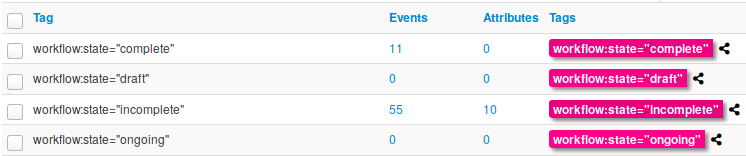
\includegraphics[width=1.0\linewidth]{pictures/taxonomy-workflow.png}
\end{frame}

\begin{frame}
    \frametitle{Galaxies and Galaxy Clusters}
    \begin{itemize}
        \item[\textbf{Galaxy}] Container to group galaxy clusters of the same type
        \item[\textbf{Galaxy Cluster}] knowledge-base item with complex meta-data aimed for human consumption
    \end{itemize}
    \begin{itemize}
        \item Community driven \textbf{knowledge-base libraries used as tags}
        \item Including descriptions, links, synonyms, meta information, etc. 
        \item \textbf{Flexible} and \textbf{reusable}
        \item Works the exact same way as taxonomies but with more meta-data
        \begin{itemize}
            \item \texttt{misp-galaxy:ransomware="CryptoLocker"}
            \item Contains description, reference, documentation and other meta-data
        \end{itemize}
    \end{itemize}
    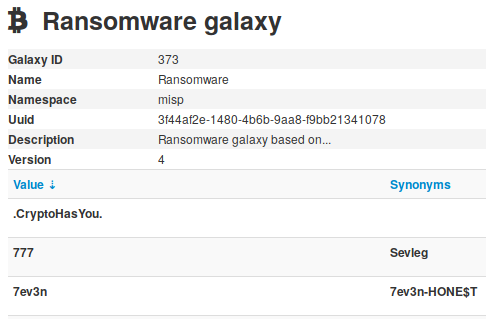
\includegraphics[scale=1.0]{pictures/galaxy-ransomware.png}
\end{frame}

\begin{frame}
    \frametitle{MITRE ATT\&CK and Galaxy Matrices}
    \begin{itemize}
        \item MITRE ATT\&CK is one of the best knowledge base of adversary TTPs
        \item Widely used and supported by a lot of tools
        \item The catalogue includes a matrix-like interface
        \item Offers clear visualisation for the kill chain
    \end{itemize}
    \note[item]{The kill chain are the sequential steps that adversaries can perform in order to achieve an attack}
    \begin{itemize}
        \item MISP Fully support ATT\&CK and embraced it's matrix structure
        \item Multiples matrix for other concerns are available:
        \begin{itemize}
            \item \texttt{Badhra} Similar to ATT\&CK but for telecom operators
            \item \texttt{attck4fraud} Regrouped clusters related to fraud actions
        \end{itemize}
    \end{itemize}
    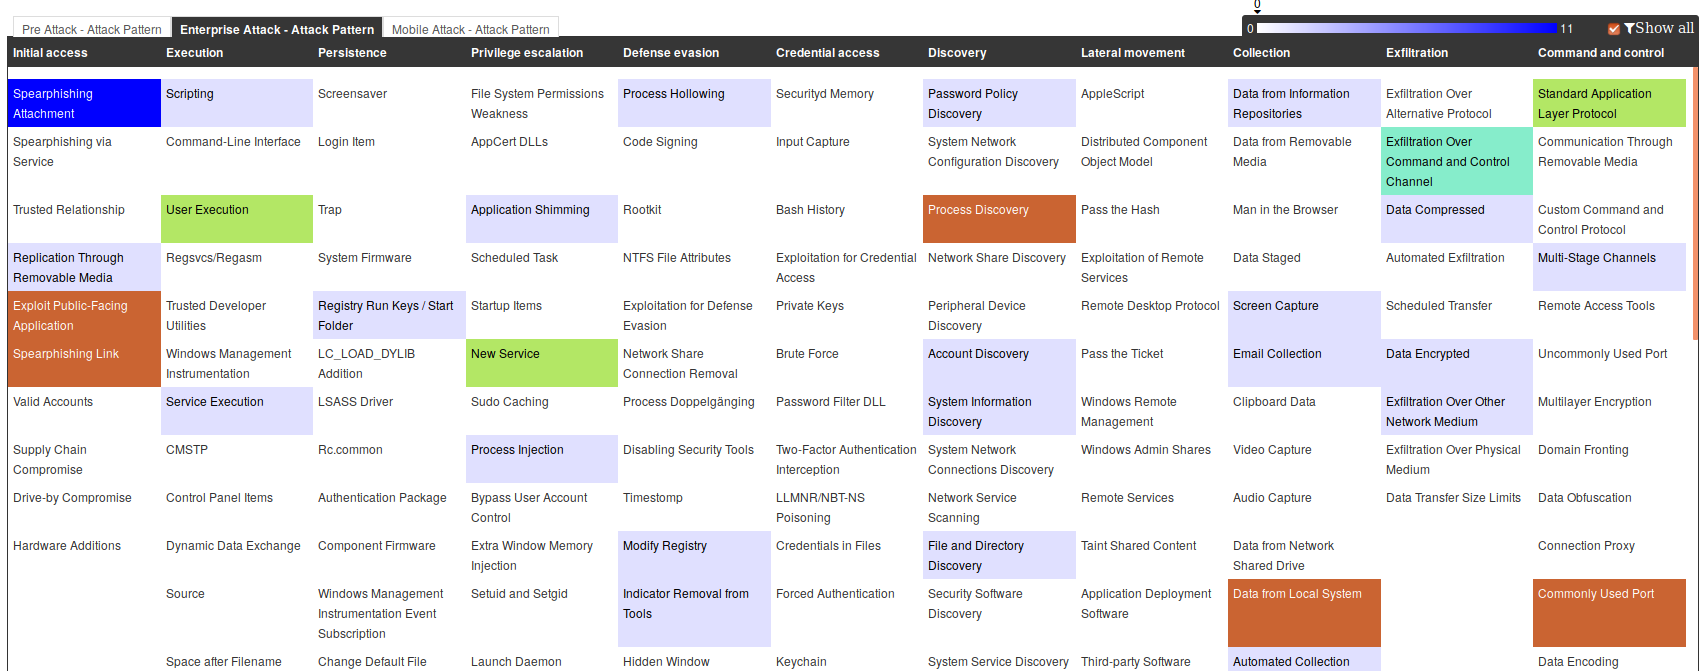
\includegraphics[scale=1.0]{pictures/attack.png}
\end{frame}

\begin{frame}
    \frametitle{MISP Objects}
    Atomic attributes are great, but are lacking a way to express that some can be related to others.

    MISP Objects are there to fill the gap:
    \begin{itemize}
        \item Template system to build complex structures composed of attributes
        \item Logically group attributes that are contextually linked between each others
        \begin{itemize}
            \item A file object can contain: a size, name, content, cryptographic hashes, etc.
            \item A car object can contain: a brand, a model, a license plate, etc.
        \end{itemize}
    \end{itemize}
    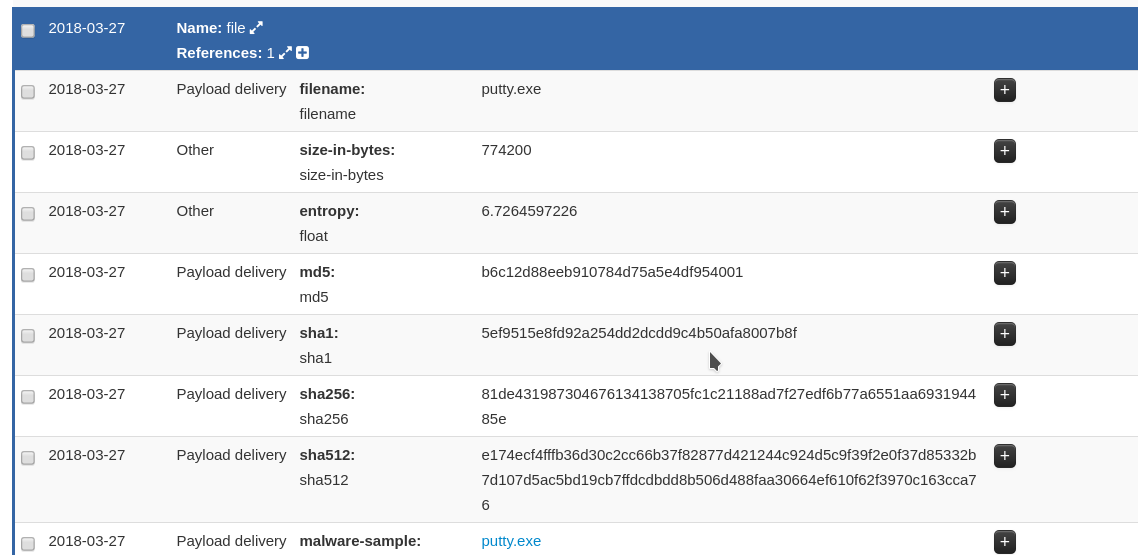
\includegraphics[scale=1.0]{pictures/object.png}
\end{frame}

\begin{frame}
    \frametitle{Relationships}
    \begin{itemize}
        \item Analysts want more than a table of atrtibute, they want to see how each of them interact with the others
        \item Relationships are essentials to describe scenarios or stories with the data
        \item MISP allow these relationship to be built between objects
    \end{itemize}
    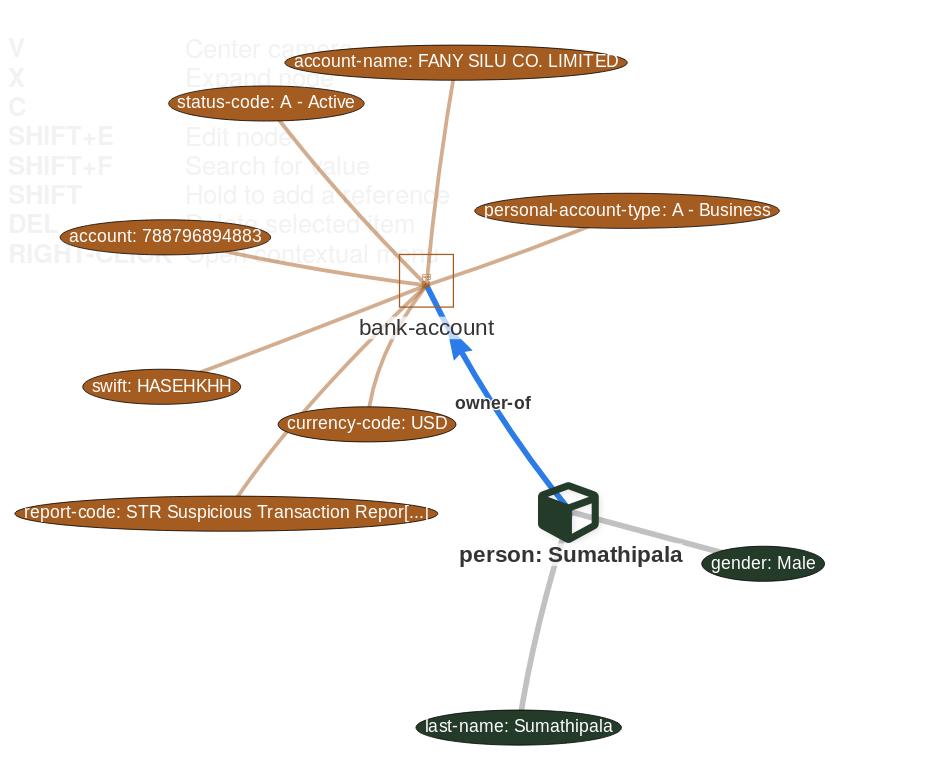
\includegraphics[scale=1.0]{pictures/relationship.png}
\end{frame}

\begin{frame}
    \frametitle{Timeliness with Sightings and \texttt{first\_seen} / \texttt{last\_seen}}
    Another aspect often neglected at first is temporality and MISP offerts to ways to avoid having the data frozen in time
    \begin{itemize}
        \item Sightings
        \begin{itemize}
            \item Allows to signal the fact that an indicator was sighted
            \item They can record the time and where they were the sighting was seen
            \item E.g.: Sight C2 servers or phishing websites
        \end{itemize}
        \item \texttt{first\_seen} / \texttt{last\_seen}
        \begin{itemize}
            \item These two data-points allow to set when the specified item was first and last seen
            \item Enables the visualisation of data timeframe with a timeline
            \item E.g.: Track the duration of a campaign or duration for which something was online
        \end{itemize}
        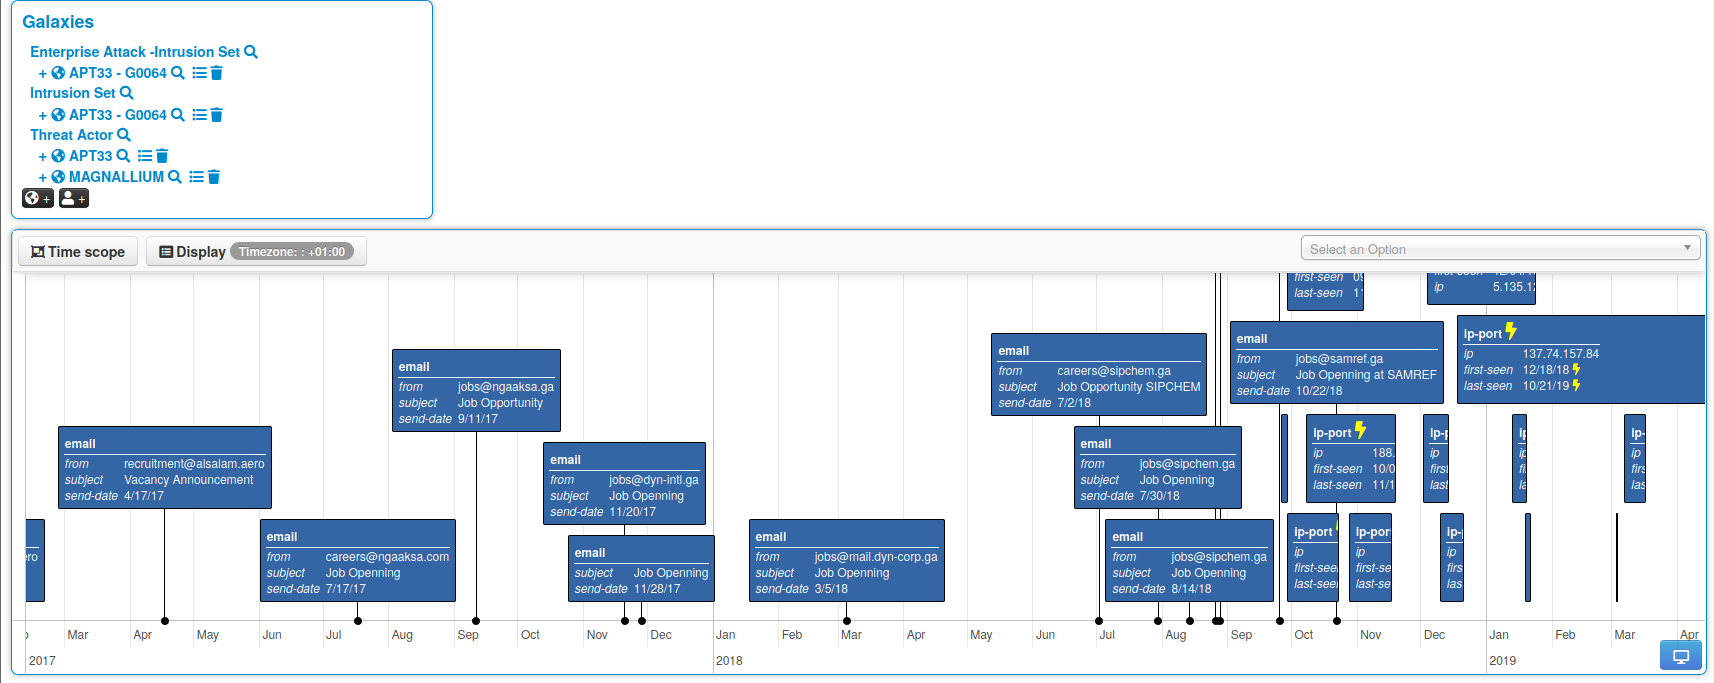
\includegraphics[scale=1.0]{pictures/timeline.png}
    \end{itemize}
\end{frame}

\section{Best practises to encode and contextualise}
\begin{frame}
    \frametitle{Encoding: Event}
    Always keep in mind that the recipient is a human:
    \begin{itemize}
        \item Include a self-explanatory title
        \item Make it concise
        \item Include a report (using event-report) along with the machine parsable data
    \end{itemize}
    That will make the live of the analyst easier: That analyst might end up being you!
\end{frame}

\begin{frame}
    \frametitle{Encoding: Attributes and objects}
    Atomic data by themselve rarely exists: They are often linked to another entity
    \begin{itemize}
        \item Interactions between between elements are frequent
        \begin{itemize}
            \item They can often be described by using verbs: \texttt{connects-to}, \texttt{contain-within}, ...
        \end{itemize}
        \item A story can be inferred without the need to put it into words
        \begin{itemize}
            \item \texttt{file} was attached to \texttt{email} which when extracted contained a \texttt{malware} connecting to \texttt{ip-address} which was used \texttt{C2}
        \end{itemize}
        \item Properly encoding these relationships turns flat data into a connected graph
    \end{itemize}
\end{frame}


\begin{frame}
    \frametitle{Contextualise: Distributions and permissible actions}
    Adding context on what actions can be done on the data and who can it be shared with
    \begin{itemize}
        \item Permissible actions taxonomies:
        \begin{itemize}
            \item \texttt{PAP}: Permissible Actions Protocol
            \item \texttt{IEPF}: Information Exchange Policy (IEP) Framework
        \end{itemize}
        \item Sharing level taxonomies:
        \begin{itemize}
            \item \texttt{TLP}: Traffic Light Protocol
            \item \texttt{IEPF}: Information Exchange Policy (IEP) Framework
        \end{itemize}
    \end{itemize}
\end{frame}

\begin{frame}
    \frametitle{Contextualise: Attributes and their context}
    Each data point has a meaning and tells a part of the story:
    \begin{itemize}
        \item In what context was this IoC seen?
        \item Is it related to compromision? Does it tell us anything about the adversary infrastructure
        \item Was it used to exfiltrate data? Did it acted as a C2?
        \item Did it perform subsequent actions?
        \item ATT\&CK can procure even more knowledge
    \end{itemize}

    However, think twice before tagging:
    \begin{itemize}
        \item If a tag applies to the whole content of the event, it should be attached on the event instead
        \item If the tag offers no real utility or hinder your ability to analyse the whole dataset, it should probably be ignored
    \end{itemize}
\end{frame}

\begin{frame}
    \frametitle{Contextualise: Origin, likelyhood and reliability}
    \begin{itemize}
        \item The source of information has an impact on how people evaluates its trust
        \begin{itemize}
            \item Data without its source/origin might be considered unreliable by default
            \item i.e: A research paper without citing its sources is useless
        \end{itemize}
        \item MISP bridge people and and communities
        \begin{itemize}
            \item The more one is connected, the greqter the quantity and diversity of data
            \item Not everything you read on the internet is true
        \end{itemize}
    \end{itemize}

    If you can't share the source, provide the trust in the source
    \begin{itemize}
        \item Include the reliability and the credibility of the information
            \begin{itemize}
                \item Taxonomy: \texttt{admiralty-scale}
                \item i.e: \texttt{admiralty-scale:source-reliability="Usually reliable"}
            \end{itemize}
        \item Include the quality and likelyhood
            \begin{itemize}
                \item Taxonomy: \texttt{estimative-language}
                \item i.e: \texttt{estimative-language:likelihood-probability="very-likely"}
            \end{itemize}
    \end{itemize}
\end{frame}

\begin{frame}
    \frametitle{Contextualise: Make the attribution}
    \begin{itemize}
        \item The purpose is not to blame but to identity the attacker's intent
        \item Knowing the intent greatly help to:
        \begin{itemize}
            \item Know the objectives
            \item Understand what are the target assets
            \item Deduce the treat level
        \end{itemize}
        \item Allow to identity behaviors
        \begin{itemize}
            \item Might speed up the next investigation
            \item Might boostrap the analysis procdess
        \end{itemize}
    \end{itemize}
\end{frame}

\begin{frame}
    \frametitle{Contextualise: Provide advices on how to protect themselves}
    \begin{itemize}
        \item Indicate what can be done with the data
        \begin{itemize}
            \item Use it to feed an IDS
            \item Perform historical search with a SIEM to find potential compromision
            \item Inform your peers against a new type of threat
        \end{itemize}
        \item Provide additional supporting materials
        \begin{itemize}
            \item The original report form which the data is coming from
            \item Home-brew scripts
            \item Sigma rules for SIEM searches
            \item Context and configurations under which the analysis was done
        \end{itemize}
    \end{itemize}
\end{frame}


\section{How can context be leveraged}
\begin{frame}[fragile]
    \frametitle{Advanced ways of querying data}
    Let's make use of this well-structured, context-rich data
    \begin{itemize}
        \item Incorporate all contextualisation options into API filters
    \end{itemize}
\begin{lstlisting}
{
    "AND": [
        "admiralty-scale:source-reliability=\"Reliable\""
    ],
    "OR": [
        "threat-actor=\"Sofacy\"",
        "sector=\"Chemical\"",
        "country=\"Luxembourg\"",
    ]
}
\end{lstlisting}

    \begin{itemize}
        \item On-demande potential false positive exclusion
        \begin{itemize}
            \item Warninglist system helps to exclude known false-positives reducing alert-fatigue
        \end{itemize}
        \item IoC prioritization and lifecycle management
        \begin{itemize}
            \item Integrate decay models to filter out expired/unrelevant data
        \end{itemize}
        \item Allow users to build their own export module
    \end{itemize}
\end{frame}

\begin{frame}
    \frametitle{Enabling common user profiles to better perform their tasks}
    How does different user profiles benefits to most of well-structured, context-rich data
    \begin{itemize}
        \item[\textbf{incident responder}]: Self-explanatory data relieves pressure and reduces the change of misunderstanding it
        \item[\textbf{SOC operator}]: Reduce alert-fatigue and energy to filter unwanted data
        \item[\textbf{ISP}]: Ease the task to decide if the data is fit for blocking based on trust and context the data was seen in
        \item[\textbf{threat analyst}]: Provide insight on the modus operandi and goals of attacker
        \item[\textbf{risk analyst}]: Help highlighting potential security gaps and formulate advices on preventive actions
        \item[\textbf{decision maker}]: Guide resources allocation based on current/emerging threats for their region and sector
    \end{itemize}
\end{frame}


\section{How to structure non-technical information}
\begin{frame}
    \frametitle{Objectives}
    \begin{itemize}
        \item Identify non-technical data that can be useful for an investigation,
        \item Illustrate how non-technical and technical data can interact to produce meaninful insights,
        \item Model these interactions,
        \item Outline what Socio-Technical intercations are useful to share.
    \end{itemize}

    \note[item]{A note for the slide handout}
\end{frame}


\begin{frame}
    \frametitle{We live in Socio-Technical Systems}
    Computer and their security is linked to human activities:

    \begin{itemize}
        \item Technical traces show human activities,
        \item Technical traces can convey human intent,
        \item Human interactions can explain and give context to Technical traces,
        \item CyberCrime requires infrastructures and logistics that are discussed between humans,
        \item TTPS are discussed and exchanged,
        \item Human interaction can help attributing an attack,
        \item Human interaction can help deciphering intent and motives, and discriminate human error from sabotage.
    \end{itemize}
    \note[item]{A note for the slide handout}
\end{frame}


\begin{frame}
    \frametitle{Plan}
    \begin{itemize}
        \item Modeling a specific ransomware case,
        \item Using OSINT and data leaks to bring context to other ransomware cases.
    \end{itemize}

    \note[item]{A note for the slide handout}
\end{frame}

\section{Conti analysis}


\begin{frame}[fragile]
    \frametitle{Ransomware Jabber chats leak}
    Published on Twitter:
    \begin{figure}[t]
        
\includegraphics[width=.8\textwidth]{contileaks-twitter.png}
        \centering
    \end{figure}

    Contained XMPP server logs:
    \begin{figure}[t]
        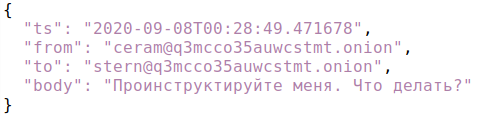
\includegraphics[width=.6\textwidth]{contileaks-json.png}
        \centering
    \end{figure}
\end{frame}


\begin{frame}[fragile]
    \frametitle{Ransomware Jabber chats leak}
    Our goal is:
    \begin{itemize}
        \item Dig into these Jabber chats in search for IoC and operational information
        \item use MISP to correlate this information from past cases,
        \item ease attribution of these past cases through IoC,
        \item add context to past cases from the chats logs in order to ease their investigation,
        \item support colleagues and other CSIRTs with real Intelligence.
    \end{itemize}
\end{frame}

\begin{frame}
    \frametitle{Ransomware Jabber chats leak}
    We use AIL\footnote{\url{https://ail-project.org/}} to dig into the data:
    \begin{itemize}
        \item AIL processes the data and search for relevant information
        \begin{itemize}
        \item PGP keys,
        \item Bitcoin addresses, maybe others,
        \item onion hidden services.
        \end{itemize}
    \item Once we find relevant information we push it into MISP,
    \item we use MISP correlation engine to find relevant past cases.
    \end{itemize}
    TODO: checking if the data we have actually allows that
    \note[item]{A note for the slide handout}
\end{frame}

\begin{frame}
    \frametitle{To sum it all up}
    \begin{itemize}
        \item Given the growth and diversification and matury or users, contextualisation is becoming essential
        \item Well-structured, context-rich data is good as it enables better decision making
        \item It will rise user capabilities and thus improve protection
        \item MISP has a format and tools designed to support contextualised data
    \end{itemize}
\end{frame}

\begin{frame}
    \frametitle{Acknowledgment}
    Add your sources!
    \begin{itemize}
        \item \texttt{Turning data into actionable intelligence - advanced features in MISP supporting your analysts and tools} (CIRCL.lu)
        \begin{itemize}
            \item \url{https://www.enisa.europa.eu/events/2019-cti-eu/2019-cti-eu-bonding-eu-cyber-threat-intelligence}
        \end{itemize}
        \item \texttt{Colouring Outside the Lines} (Andras Iklody \& Trey Darley)
        \begin{itemize}
            \item \url{https://www.first.org/conference/2020/recordings}
        \end{itemize}
        \item MISP Training Materials
        \begin{itemize}
            \item \url{https://github.com/MISP/misp-training}
        \end{itemize}
    \end{itemize}
\end{frame}